%% This is file `elsarticle-template-1-num.tex',
%%
%% Copyright 2009 Elsevier Ltd
%%
%% This file is part of the 'Elsarticle Bundle'.
%% ---------------------------------------------
%%
%% It may be distributed under the conditions of the LaTeX Project Public
%% License, either version 1.2 of this license or (at your option) any
%% later version.  The latest version of this license is in
%%    http://www.latex-project.org/lppl.txt
%% and version 1.2 or later is part of all distributions of LaTeX
%% version 1999/12/01 or later.
%%
%% Template article for Elsevier's document class `elsarticle'
%% with numbered style bibliographic references
%%
%% $Id: elsarticle-template-1-num.tex 149 2009-10-08 05:01:15Z rishi $
%% $URL: http://lenova.river-valley.com/svn/elsbst/trunk/elsarticle-template-1-num.tex $
%%
\documentclass[preprint,12pt]{elsarticle}

%% Use the option review to obtain double line spacing
%% \documentclass[preprint,review,12pt]{elsarticle}

%% Use the options 1p,twocolumn; 3p; 3p,twocolumn; 5p; or 5p,twocolumn
%% for a journal layout:
%% \documentclass[final,1p,times]{elsarticle}
%% \documentclass[final,1p,times,twocolumn]{elsarticle}
%% \documentclass[final,3p,times]{elsarticle}
%% \documentclass[final,3p,times,twocolumn]{elsarticle}
%% \documentclass[final,5p,times]{elsarticle}
%% \documentclass[final,5p,times,twocolumn]{elsarticle}

%% The graphicx package provides the includegraphics command.
\usepackage{graphicx}
%% The amssymb package provides various useful mathematical symbols
\usepackage{amssymb}
%% The amsthm package provides extended theorem environments
%% \usepackage{amsthm}

%% The lineno packages adds line numbers. Start line numbering with
%% \begin{linenumbers}, end it with \end{linenumbers}. Or switch it on
%% for the whole article with \linenumbers after \end{frontmatter}.
\usepackage{lineno}

%% natbib.sty is loaded by default. However, natbib options can be
%% provided with \biboptions{...} command. Following options are
%% valid:

%%   round  -  round parentheses are used (default)
%%   square -  square brackets are used   [option]
%%   curly  -  curly braces are used      {option}
%%   angle  -  angle brackets are used    <option>
%%   semicolon  -  multiple citations separated by semi-colon
%%   colon  - same as semicolon, an earlier confusion
%%   comma  -  separated by comma
%%   numbers-  selects numerical citations
%%   super  -  numerical citations as superscripts
%%   sort   -  sorts multiple citations according to order in ref. list
%%   sort&compress   -  like sort, but also compresses numerical citations
%%   compress - compresses without sorting
%%
%% \biboptions{comma,round}

% \biboptions{}

\journal{Journal Name}

\pdfoutput=1
\usepackage[latin1]{inputenc}
\usepackage{amsmath}
\usepackage{amssymb}
\usepackage{color}

\usepackage{mathtools}
\usepackage{float}
\usepackage{hyperref}
\usepackage[T1]{fontenc}

\def\ket#1{|#1\rangle}
\def\e#1{ e^{#1}}
\def\bra#1{\langle#1|}
\def\av#1{\langle#1\rangle}

\def\tder#1{\frac{d#1}{dt}}
\def\eps{\varepsilon}
\def\nup{\nu^\prime}

\def\aop{\hat{a}}
\def\adop{\hat{a}^\dagger}
\def\awop{\tilde{a}}
\def\awdop{\tilde{a}^\dagger}
\def\bop{\hat{b}}
\def\bwop{\tilde{b}}
\def\bwdop{\tilde{b}^\dagger}
\def\cop{\hat{c}}
\def\cwop{\tilde{c}}
\def\cwdop{\tilde{c}^\dagger}
\def\Xop{\hat{X}}
\def\Xwop{\tilde{X}}
\def\Hop{\hat{H}}
\def\nuop{\hat{\nu}}
\def\xiop{\hat{\xi}}
\def\xidop{\hat{\xi}^\dagger}
\def\xiwop{\tilde{\xi}}
\def\xiwdop{\tilde{\xi}^\dagger}
\def\thetap{{\theta^\prime}}
\def\mnu{{-\nu}}
\def\sm{{-}}
\def\refeq#1{{\hyperref[#1]{(\ref*{#1})}}}
\def\reffig#1{{\hyperref[#1]{FIG. \ref*{#1}}}}
\def\refsec#1{{\hyperref[#1]{SEC. \ref*{#1}}}}
\def\refno#1{{\hyperref[#1]{\ref*{#1}}}}


\def\nn{\nonumber}

\newcommand{\lsz}{\left[}
\newcommand{\rsz}{\right]}
\newcommand{\lk}{\left(}
\newcommand{\rk}{\right)}
\newcommand{\lka}{\left\{}
\newcommand{\rka}{\right\}}
\newcommand{\labs}{\left|}
\newcommand{\rabs}{\right|}
\pdfminorversion=4

\newcommand{\gguide}{{\it NDPA paper}}
%Uncomment next line if AMS fonts required
%\usepackage{iopams}  
\begin{document}

\begin{frontmatter}

\title{Enhancement of EPR-type entanglement in an NDPA with coherent time-delayed feedback}

\author{Nikolett N\'emet and Scott Parkins}

\address{University of Auckland, Department of Physics and The Dodd-Walls Centre for Photonics and Quantum Technologies}
\ead{nnem614@aucklanduni.ac.nz}
\begin{abstract}
This paper presents an analysis on the effects of coherent time-delayed feedback of the down-converted fields in a Nondegenerate Parametric Amplifier. We observe enhanced Einstein-Podolsky-Rosen type of entanglement between the two modes at a given driving strength. Increased correlation can be shown both on resonance and at shifted frequencies due to the finite time-delay in the feedback loops.
\end{abstract}
\end{frontmatter}
%Uncomment for PACS numbers title message
%\pacs{00.00, 20.00, 42.10}
% Keywords required only for MST, PB, PMB, PM, JOA, JOB? 
%\vspace{2pc}
%\noindent{\it Keywords}: Article preparation, IOP journals
% Uncomment for Submitted to journal title message
%\submitto{\JPA}
% Comment out if separate title page not required
\linenumbers

\section{Introduction}

In the most general case the mirrors of the cavity have different transmission rate for each down-converted mode ($\kappa_{1/2,a/b}$).
picked up as a result of the frequency difference, reflections and other processes is included in the phase factors $\phi_{a,b}$

\cite{Nemet2016}
\begin{figure}[h!]
\centering
%\vglue -.2 cm
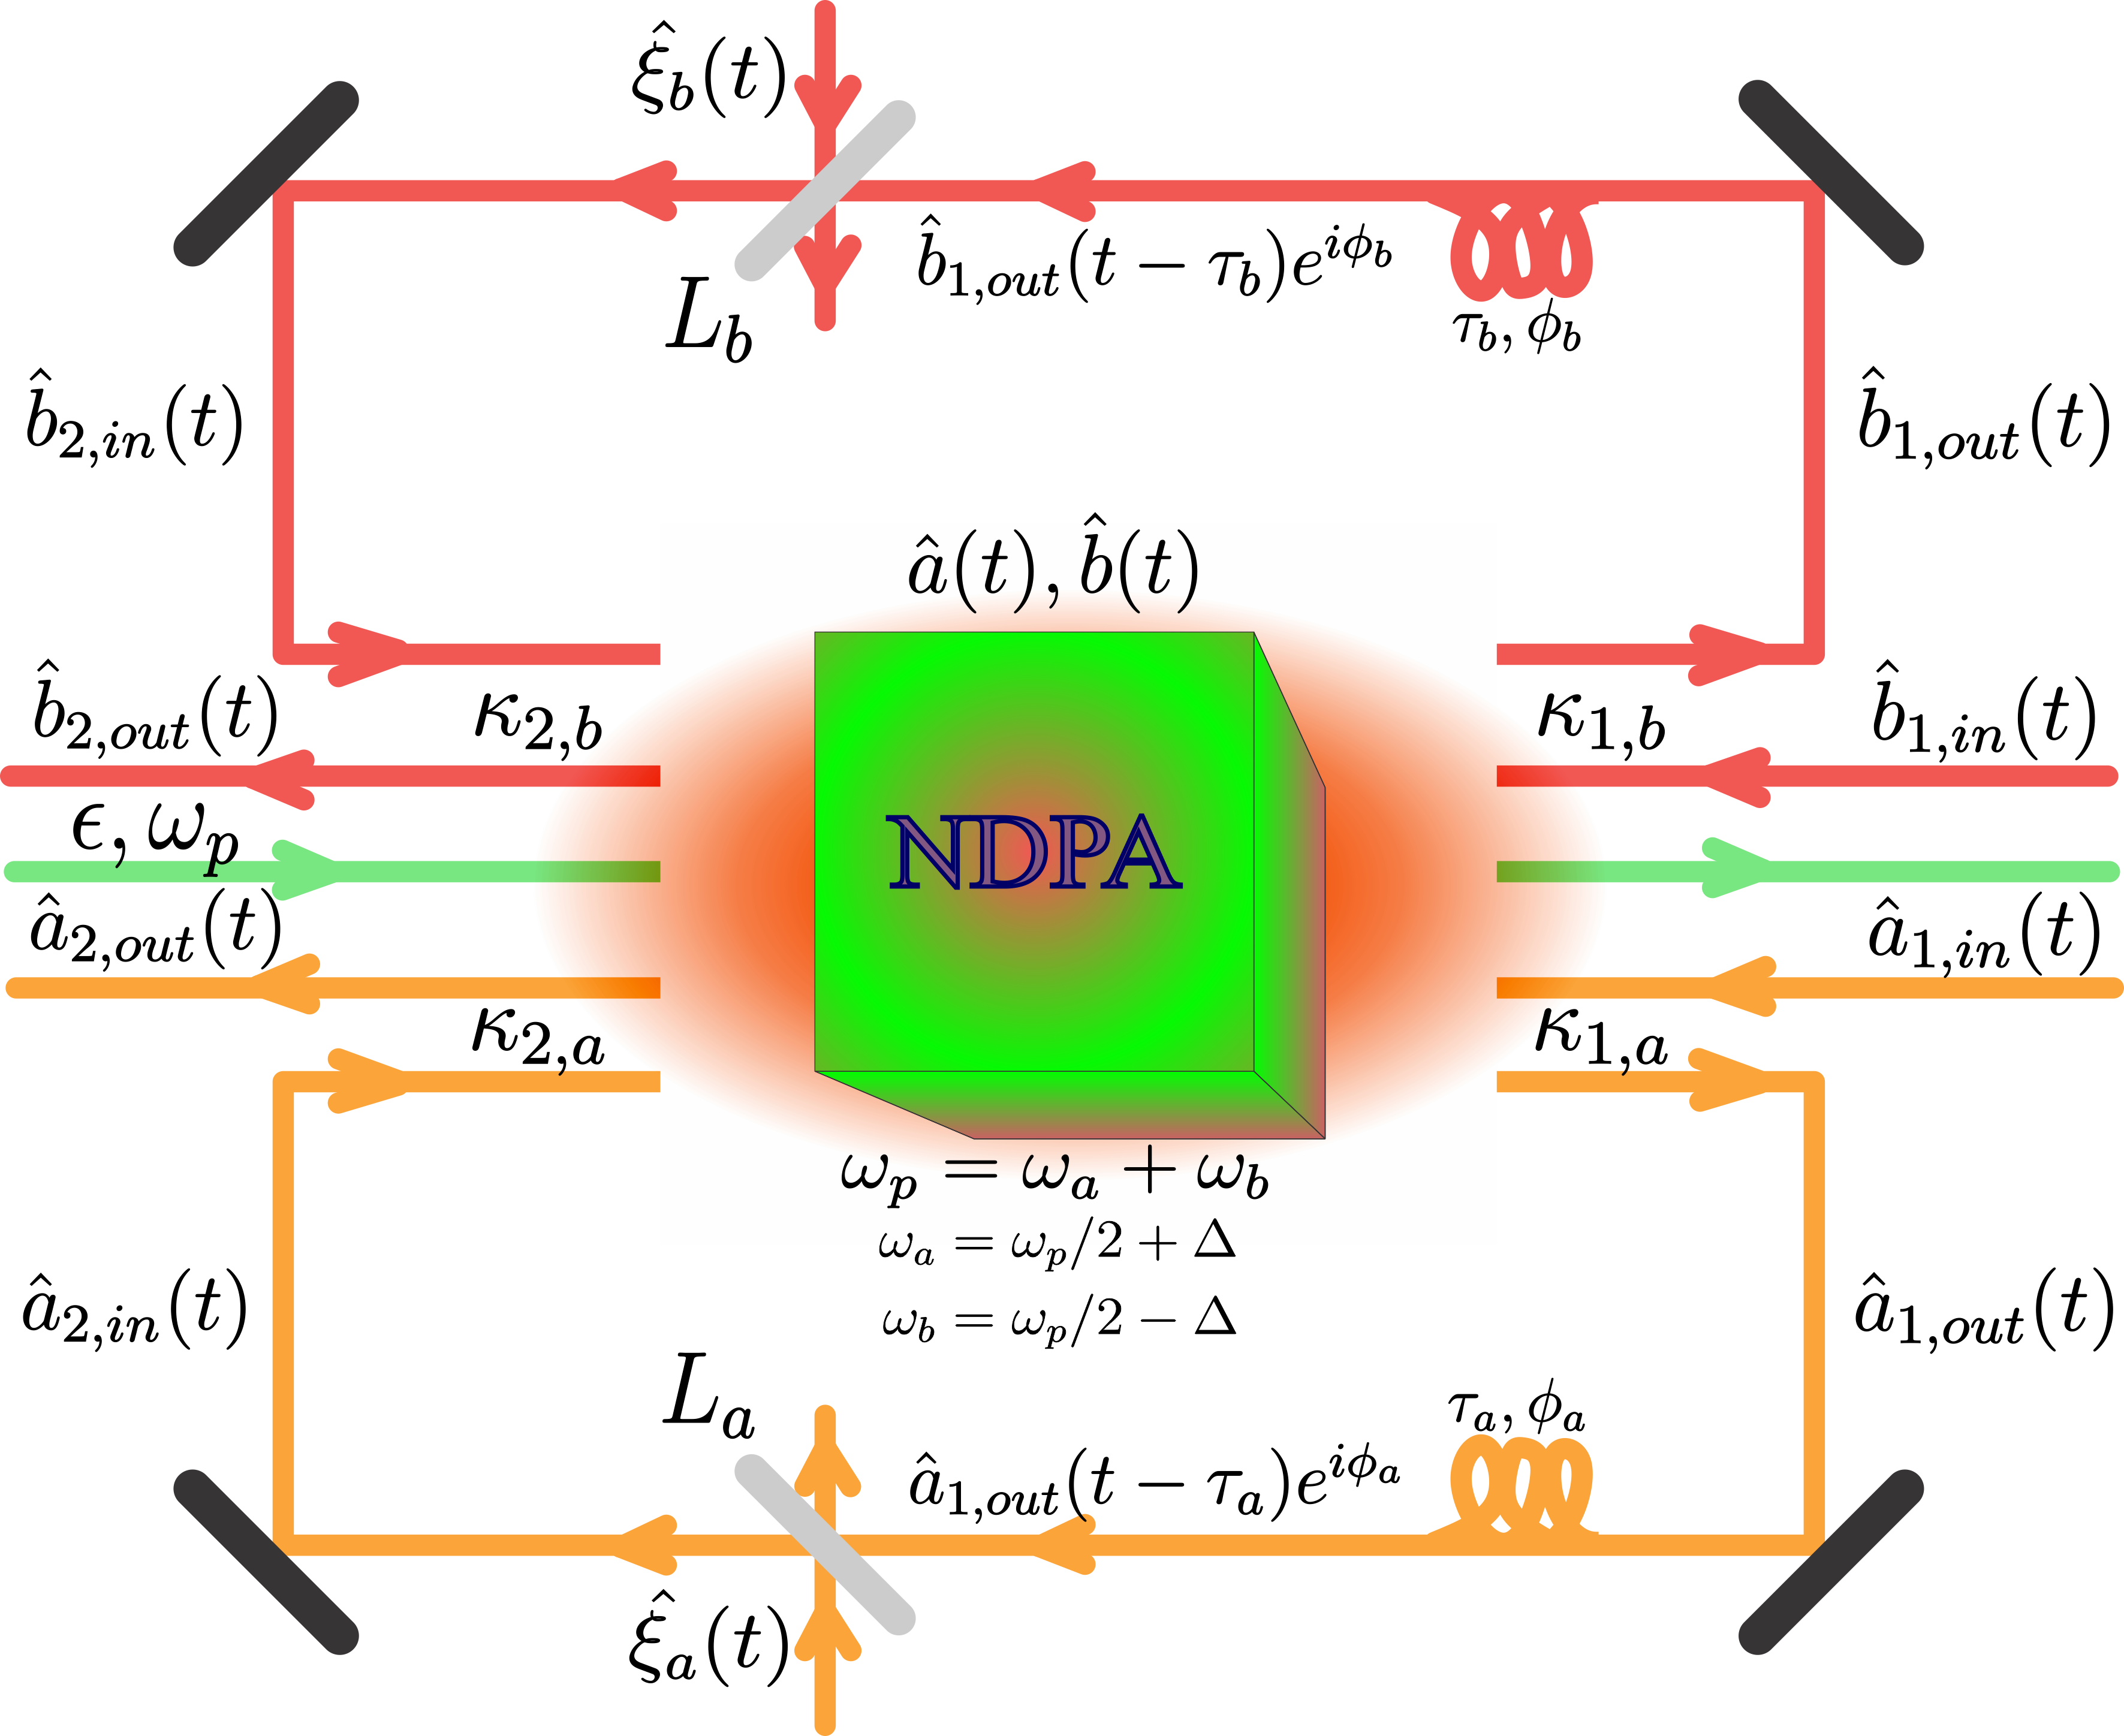
\includegraphics[width=.75\textwidth]{figure1.png}
%\vglue -1 cm
\textit{\textbf{\caption{\linespread{1}\small{Schematic setup. The nonlinear crystal performing parametric down-conversion on the incoming photons is placed in a cavity. The output fields on the right hand side is directly coupled back into the input channels of the other side without performing any measurement. The longer length of the loops support a finite time-delay in the feedback loop ($\tau_{a,b}$) and phase shift ($\phi_{a,b}$). Losses are also incorporated in the feedback loop with a beam splitter model.}}}}
%\vglue -.3 cm
\end{figure}

\section{EPR-type entanglement in NDPA}
\section{Without time-delay}
\section{With time-delay}
\section{Differences in the loops}

\section*{References}
\bibliographystyle{apsrev4-1}
\bibliography{NDPA}

\end{document}